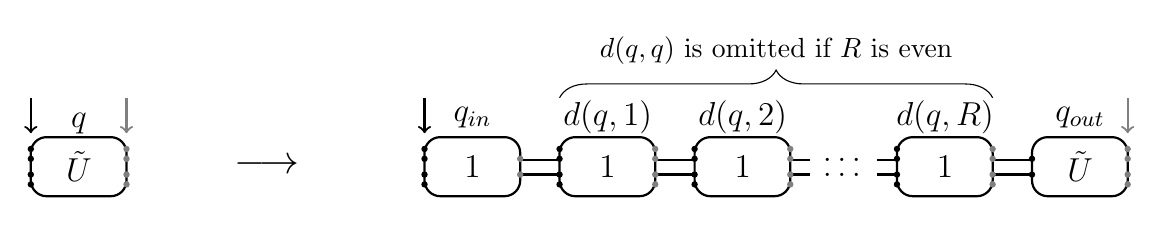
\begin{tikzpicture}[scale=0.5]
\begin{scope}[xshift=-10 cm]       
\draw[rounded corners=2mm,thick] (0,0) rectangle (2.43cm,1.5 cm);  
  \foreach \x /\color in {0/black,2.43/gray}
{     \foreach \y in {1.2,.95,.55,.3}
{       \draw[fill=\color,draw=\color] (\x cm, \y cm) circle (.66mm);
    }} 
\node at (1.22cm, .75cm) {\large{$\tilde U$}};   
 \node at (1.22cm, 1.85cm){\large{$q$}};

\node at (6cm, 0.75cm) {\Large{$\longrightarrow$}};
\draw [->, thick, color=black] (0,2.5) --(0,1.6);
\draw [->, thick, color=gray] (2.43,2.5) --(2.43,1.6);
\end{scope}
\draw [decorate,decoration={brace,amplitude=10pt}] (3.43,2.5) -- (14.43,2.5) node [black,midway,yshift=17]  {$d(q,q)$ is omitted if $R$ is even};
\draw [->, thick, color=black] (0,2.5) --(0,1.6);
\draw [->, thick, color=gray] (17.86,2.5) --(17.86,1.6);
  % The connections 
 \foreach \y in {0.925,.55}{  
  \draw[thick] (2.43,\y) -- (3.43,\y);
	\draw[thick] (5.86,\y) -- (6.86,\y);	
	\draw[thick] (14.43,\y) -- (15.43,\y);
	\draw[thick] (9.29,\y) -- (9.79,\y);
	\draw[thick] (11.5,\y) -- (12,\y);
	\node at (10.6,\y){\large{$\ldots$}};
}
%\draw[thick,looseness = 200] (0,1.2) to [out = 180, in = 100] (-.01,1.2);
  % The two rectangles 

%  15.43/\tilde U/q_{\mathrm{out}}
\draw[rounded corners=2mm,thick] (0,0) rectangle (2.43cm,1.5 cm);  
{     \foreach \y in {1.2,.95,.55,.3}
{       \draw[fill=black,draw=black] (0 cm, \y cm) circle (.66mm);
  }} 
  {     \foreach \y in {.95,.55}
{       \draw[fill=gray,draw=gray] (2.43 cm, \y cm) circle (.66mm);
  }} 
  \node at (1.22cm, .75cm) {\large{$1$}};   
 \node at (1.22cm, 2cm){\large{$q_{\text{in}}$}};   
 
 
 \begin{scope}[xshift=15.43 cm]
 \draw[rounded corners=2mm,thick] (0,0) rectangle (2.43cm,1.5 cm);  
{     \foreach \y in  {.95,.55}
{       \draw[fill=black,draw=black] (0 cm, \y cm) circle (.66mm);
  }} 
  {     \foreach \y in{1.2,.95,.55,.3}
{       \draw[fill=gray,draw=gray] (2.43 cm, \y cm) circle (.66mm);
  }} 
  \node at (1.22cm, .75cm) {\large{$\tilde{U}$}};   
 \node at (1.22cm, 2cm){\large{$q_{\text{out}}$}};   
 \end{scope}
 
 % the inner d(q,s) 
 \foreach \offset/\unitary/\label in {3.43/1/{d(q,1)},6.86/1/{d(q,2)},12/1/{d(q,R)}}
{   
\begin{scope}[xshift=\offset cm]       
\draw[rounded corners=2mm,thick] (0,0) rectangle (2.43cm,1.5 cm);  
  \foreach \x /\color in {0/black,2.43/gray}
{     \foreach \y in {1.2,.95,.55,.3}
{       \draw[fill=\color,draw=\color] (\x cm, \y cm) circle (.66mm);
    }} 
  \node at (1.22cm, .75cm) {\large{$\unitary$}};   
 \node at (1.22cm, 2cm){\large{$\label$}};   
\end{scope}}   
\end{tikzpicture}